% !TeX root = ../main.tex
\subsection{Hi-C matrices} \label{chap: Hi-C matrices}

Hi-C maps are useful tools to detect the interactions occuring inside a genome in analysis. Indeed, it allows to gain insights about the stuctural disposition of chromatin domains, loops and regions.
\cite{lajoieHitchhikerGuideHiC2015}.
The experimental procedure is described in figure \ref{fig: HiC sequencing}. Each position, written as a touple (\textit{i}, \textit{j})  in a Hi-C matrix, such as the one in figure ... %#TODO add figures after optimization
represent the number of contacts between the position $i^{\text{th}}$ and $j^{\text{th}}$. The resolution of an Hi-C map will be dependent on the sequencing process, and have to be decided on the base of the type of information that we want to recover from the data
\cite{lajoieHitchhikerGuideHiC2015}.

\begin{figure}[H]
    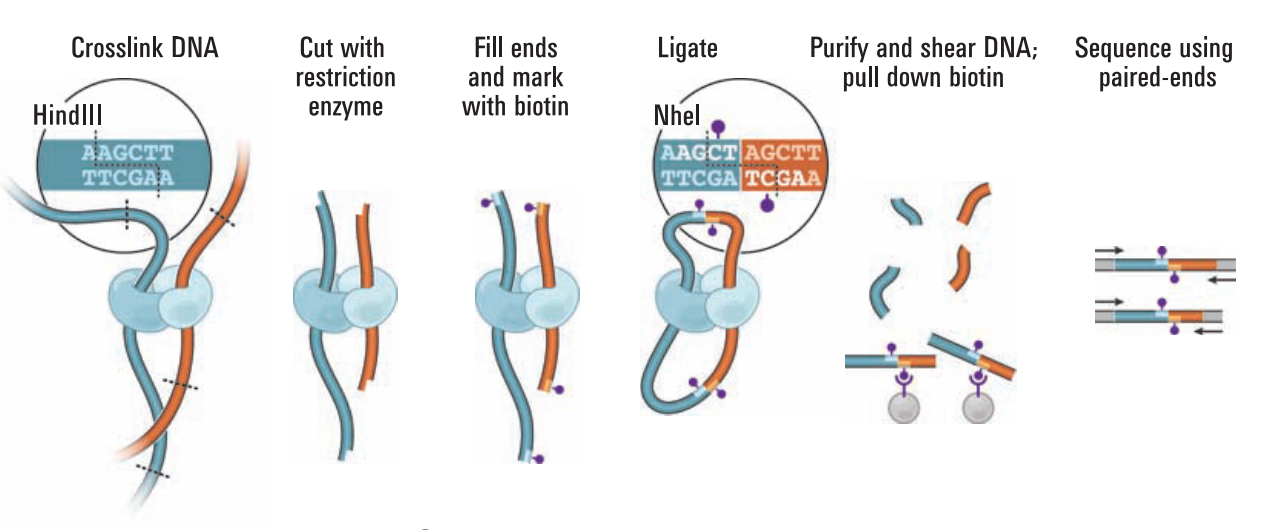
\includegraphics[width=0.75\linewidth]{./images/HiC-seq.png}
    \caption{Image taken from the following \href{https://data.4dnucleome.org/experiment-types/dilution-hi-c/}{link}
    \cite{lieberman-aidenComprehensiveMappingLong2009}, 
    representing the Hi-C sequencing technique in a schematized way.}
    \label{fig: HiC sequencing}
\end{figure}

The following list of patterns can be found by inspecting an Hi-C matrix
\cite{distefanoHiCconstrainedPhysicalModels2016,lajoieHitchhikerGuideHiC2015}.

\begin{enumerate}
    \item \textbf{Cis/trans interaction ratio}: Those interactions manifest themselves in square blocks. There are higher interaction frequencies on average between pairs of \textit{loci} in the same chromosome (\textit{cis}), with respect to those among \textit{loci} which reside on different chromosomes (\textit{trans}). The viewed specificity could be a direct consequence of the presence of genomic territories. The ratio between \textit{cis/trans} interactions could be indicative of the quality of the obtained data.
    
    \item \textbf{Distance-dependent interaction frequency}: From the visualization of an Hi-C matrix, it is possible to observe that the largest number of interactions are registered at small distances. On the other hand, only a few contacts can be observed with high distances. Several studies tried to predict this interesting behavior. In particular, it was found that in yeast the probability of interaction could be described with the following equation
    \cite{lajoieHitchhikerGuideHiC2015}:
    
    $$
        p_{\text{interaction}}(x,y) = Z * dist(x,y)^{-1,5}
    $$
    
    \item \textbf{Genomic compartments}: Genomic compartments have been found to be correlated with chromatin state, involving DNA accessibility, gene density, replication timing, GC content and histone marks
    \cite{lieberman-aidenComprehensiveMappingLong2009}. 
    The compartments can pertain to two categories, A and B, and are found by making a principal components analysis with the matrix generated with Pearson Correlation coefficients (a formula for it is found in chapter \ref{chap: SCC method}). In general A-type compartments are defined as the euchromatic gene-dense regions, while B compartments are defined as gene-poor heterochromatic regions. The blocks are usually 1-10 Mb long
    \cite{lajoieHitchhikerGuideHiC2015}.
    The positions where they are found depend on the cell type and biological conditions
    \cite{lajoieHitchhikerGuideHiC2015}.
    
    \item \textbf{Topological domains}: Also called TADs, they are regions with sub-Mb length, and can be visually found in Hi-C matrices as larger squared boxes. It is hypothesized that TADs specify elementary regulatory micro-environments in which promoters interact with local enhancers, and, also, some proteins like cohesins and CTCF tend to interact with the genome at the boundaries of the TADs
    \cite{lajoieHitchhikerGuideHiC2015}.
    
    \item \textbf{Point interactions}: Those are interactions occuring among small regions, and involve sequences of a few kb length. Biologically speaking, those points could indicate for example the interaction between enhancers and promoters. When considering point connections, the found value should be compared to the expected number of interactions, and the significance should be computed
    \cite{lajoieHitchhikerGuideHiC2015}.
\end{enumerate}

